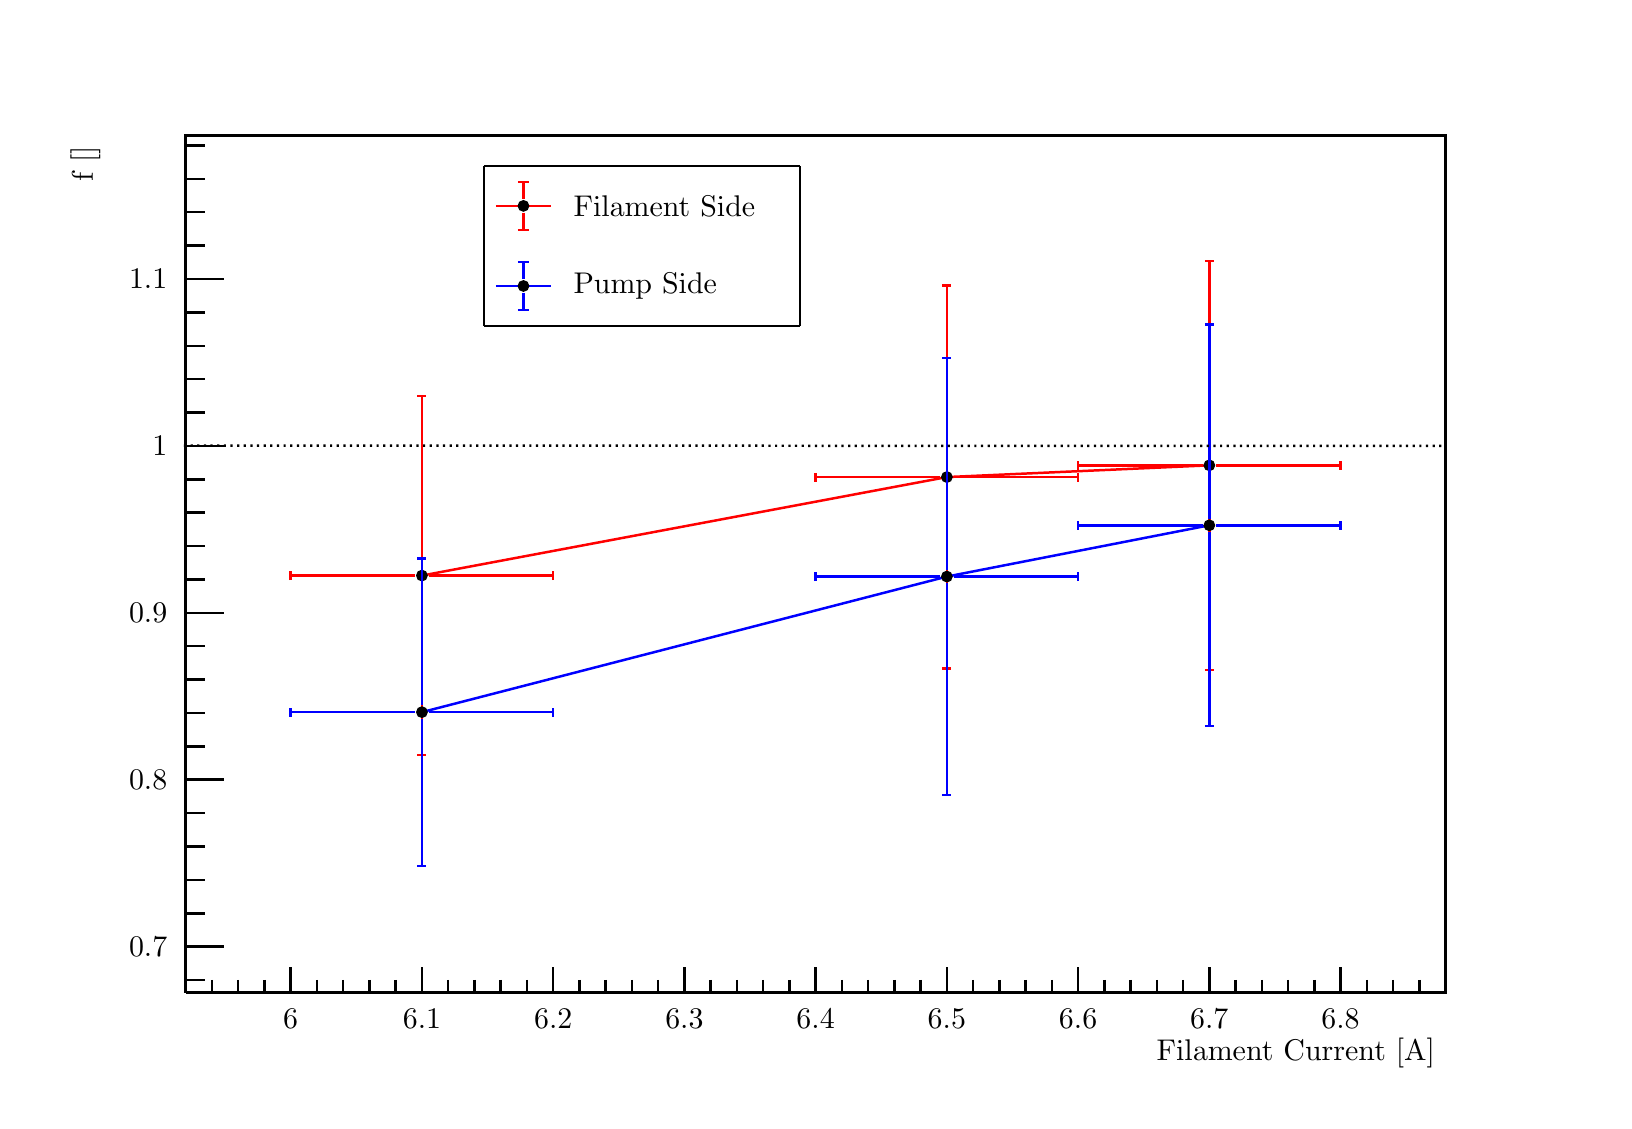
\begin{tikzpicture}
\pgfdeclareplotmark{cross} {
\pgfpathmoveto{\pgfpoint{-0.3\pgfplotmarksize}{\pgfplotmarksize}}
\pgfpathlineto{\pgfpoint{+0.3\pgfplotmarksize}{\pgfplotmarksize}}
\pgfpathlineto{\pgfpoint{+0.3\pgfplotmarksize}{0.3\pgfplotmarksize}}
\pgfpathlineto{\pgfpoint{+1\pgfplotmarksize}{0.3\pgfplotmarksize}}
\pgfpathlineto{\pgfpoint{+1\pgfplotmarksize}{-0.3\pgfplotmarksize}}
\pgfpathlineto{\pgfpoint{+0.3\pgfplotmarksize}{-0.3\pgfplotmarksize}}
\pgfpathlineto{\pgfpoint{+0.3\pgfplotmarksize}{-1.\pgfplotmarksize}}
\pgfpathlineto{\pgfpoint{-0.3\pgfplotmarksize}{-1.\pgfplotmarksize}}
\pgfpathlineto{\pgfpoint{-0.3\pgfplotmarksize}{-0.3\pgfplotmarksize}}
\pgfpathlineto{\pgfpoint{-1.\pgfplotmarksize}{-0.3\pgfplotmarksize}}
\pgfpathlineto{\pgfpoint{-1.\pgfplotmarksize}{0.3\pgfplotmarksize}}
\pgfpathlineto{\pgfpoint{-0.3\pgfplotmarksize}{0.3\pgfplotmarksize}}
\pgfpathclose
\pgfusepathqstroke
}
\pgfdeclareplotmark{cross*} {
\pgfpathmoveto{\pgfpoint{-0.3\pgfplotmarksize}{\pgfplotmarksize}}
\pgfpathlineto{\pgfpoint{+0.3\pgfplotmarksize}{\pgfplotmarksize}}
\pgfpathlineto{\pgfpoint{+0.3\pgfplotmarksize}{0.3\pgfplotmarksize}}
\pgfpathlineto{\pgfpoint{+1\pgfplotmarksize}{0.3\pgfplotmarksize}}
\pgfpathlineto{\pgfpoint{+1\pgfplotmarksize}{-0.3\pgfplotmarksize}}
\pgfpathlineto{\pgfpoint{+0.3\pgfplotmarksize}{-0.3\pgfplotmarksize}}
\pgfpathlineto{\pgfpoint{+0.3\pgfplotmarksize}{-1.\pgfplotmarksize}}
\pgfpathlineto{\pgfpoint{-0.3\pgfplotmarksize}{-1.\pgfplotmarksize}}
\pgfpathlineto{\pgfpoint{-0.3\pgfplotmarksize}{-0.3\pgfplotmarksize}}
\pgfpathlineto{\pgfpoint{-1.\pgfplotmarksize}{-0.3\pgfplotmarksize}}
\pgfpathlineto{\pgfpoint{-1.\pgfplotmarksize}{0.3\pgfplotmarksize}}
\pgfpathlineto{\pgfpoint{-0.3\pgfplotmarksize}{0.3\pgfplotmarksize}}
\pgfpathclose
\pgfusepathqfillstroke
}
\pgfdeclareplotmark{newstar} {
\pgfpathmoveto{\pgfqpoint{0pt}{\pgfplotmarksize}}
\pgfpathlineto{\pgfqpointpolar{44}{0.5\pgfplotmarksize}}
\pgfpathlineto{\pgfqpointpolar{18}{\pgfplotmarksize}}
\pgfpathlineto{\pgfqpointpolar{-20}{0.5\pgfplotmarksize}}
\pgfpathlineto{\pgfqpointpolar{-54}{\pgfplotmarksize}}
\pgfpathlineto{\pgfqpointpolar{-90}{0.5\pgfplotmarksize}}
\pgfpathlineto{\pgfqpointpolar{234}{\pgfplotmarksize}}
\pgfpathlineto{\pgfqpointpolar{198}{0.5\pgfplotmarksize}}
\pgfpathlineto{\pgfqpointpolar{162}{\pgfplotmarksize}}
\pgfpathlineto{\pgfqpointpolar{134}{0.5\pgfplotmarksize}}
\pgfpathclose
\pgfusepathqstroke
}
\pgfdeclareplotmark{newstar*} {
\pgfpathmoveto{\pgfqpoint{0pt}{\pgfplotmarksize}}
\pgfpathlineto{\pgfqpointpolar{44}{0.5\pgfplotmarksize}}
\pgfpathlineto{\pgfqpointpolar{18}{\pgfplotmarksize}}
\pgfpathlineto{\pgfqpointpolar{-20}{0.5\pgfplotmarksize}}
\pgfpathlineto{\pgfqpointpolar{-54}{\pgfplotmarksize}}
\pgfpathlineto{\pgfqpointpolar{-90}{0.5\pgfplotmarksize}}
\pgfpathlineto{\pgfqpointpolar{234}{\pgfplotmarksize}}
\pgfpathlineto{\pgfqpointpolar{198}{0.5\pgfplotmarksize}}
\pgfpathlineto{\pgfqpointpolar{162}{\pgfplotmarksize}}
\pgfpathlineto{\pgfqpointpolar{134}{0.5\pgfplotmarksize}}
\pgfpathclose
\pgfusepathqfillstroke
}
\definecolor{c}{rgb}{1,1,1};
\draw [color=c, fill=c] (0,0) rectangle (20,13.6103);
\draw [color=c, fill=c] (2,1.36103) rectangle (18,12.2493);
\definecolor{c}{rgb}{0,0,0};
\draw [c,line width=0.9] (2,1.36103) -- (2,12.2493) -- (18,12.2493) -- (18,1.36103) -- (2,1.36103);
\definecolor{c}{rgb}{1,1,1};
\draw [color=c, fill=c] (2,1.36103) rectangle (18,12.2493);
\definecolor{c}{rgb}{0,0,0};
\draw [c,line width=0.9] (2,1.36103) -- (2,12.2493) -- (18,12.2493) -- (18,1.36103) -- (2,1.36103);
\draw [c,line width=0.9] (2,1.36103) -- (18,1.36103);
\draw [c,line width=0.9] (3.33333,1.68768) -- (3.33333,1.36103);
\draw [c,line width=0.9] (3.66667,1.52436) -- (3.66667,1.36103);
\draw [c,line width=0.9] (4,1.52436) -- (4,1.36103);
\draw [c,line width=0.9] (4.33333,1.52436) -- (4.33333,1.36103);
\draw [c,line width=0.9] (4.66667,1.52436) -- (4.66667,1.36103);
\draw [c,line width=0.9] (5,1.68768) -- (5,1.36103);
\draw [c,line width=0.9] (5.33333,1.52436) -- (5.33333,1.36103);
\draw [c,line width=0.9] (5.66667,1.52436) -- (5.66667,1.36103);
\draw [c,line width=0.9] (6,1.52436) -- (6,1.36103);
\draw [c,line width=0.9] (6.33333,1.52436) -- (6.33333,1.36103);
\draw [c,line width=0.9] (6.66667,1.68768) -- (6.66667,1.36103);
\draw [c,line width=0.9] (7,1.52436) -- (7,1.36103);
\draw [c,line width=0.9] (7.33333,1.52436) -- (7.33333,1.36103);
\draw [c,line width=0.9] (7.66667,1.52436) -- (7.66667,1.36103);
\draw [c,line width=0.9] (8,1.52436) -- (8,1.36103);
\draw [c,line width=0.9] (8.33333,1.68768) -- (8.33333,1.36103);
\draw [c,line width=0.9] (8.66667,1.52436) -- (8.66667,1.36103);
\draw [c,line width=0.9] (9,1.52436) -- (9,1.36103);
\draw [c,line width=0.9] (9.33333,1.52436) -- (9.33333,1.36103);
\draw [c,line width=0.9] (9.66667,1.52436) -- (9.66667,1.36103);
\draw [c,line width=0.9] (10,1.68768) -- (10,1.36103);
\draw [c,line width=0.9] (10.3333,1.52436) -- (10.3333,1.36103);
\draw [c,line width=0.9] (10.6667,1.52436) -- (10.6667,1.36103);
\draw [c,line width=0.9] (11,1.52436) -- (11,1.36103);
\draw [c,line width=0.9] (11.3333,1.52436) -- (11.3333,1.36103);
\draw [c,line width=0.9] (11.6667,1.68768) -- (11.6667,1.36103);
\draw [c,line width=0.9] (12,1.52436) -- (12,1.36103);
\draw [c,line width=0.9] (12.3333,1.52436) -- (12.3333,1.36103);
\draw [c,line width=0.9] (12.6667,1.52436) -- (12.6667,1.36103);
\draw [c,line width=0.9] (13,1.52436) -- (13,1.36103);
\draw [c,line width=0.9] (13.3333,1.68768) -- (13.3333,1.36103);
\draw [c,line width=0.9] (13.6667,1.52436) -- (13.6667,1.36103);
\draw [c,line width=0.9] (14,1.52436) -- (14,1.36103);
\draw [c,line width=0.9] (14.3333,1.52436) -- (14.3333,1.36103);
\draw [c,line width=0.9] (14.6667,1.52436) -- (14.6667,1.36103);
\draw [c,line width=0.9] (15,1.68768) -- (15,1.36103);
\draw [c,line width=0.9] (15.3333,1.52436) -- (15.3333,1.36103);
\draw [c,line width=0.9] (15.6667,1.52436) -- (15.6667,1.36103);
\draw [c,line width=0.9] (16,1.52436) -- (16,1.36103);
\draw [c,line width=0.9] (16.3333,1.52436) -- (16.3333,1.36103);
\draw [c,line width=0.9] (16.6667,1.68768) -- (16.6667,1.36103);
\draw [c,line width=0.9] (3.33333,1.68768) -- (3.33333,1.36103);
\draw [c,line width=0.9] (3,1.52436) -- (3,1.36103);
\draw [c,line width=0.9] (2.66667,1.52436) -- (2.66667,1.36103);
\draw [c,line width=0.9] (2.33333,1.52436) -- (2.33333,1.36103);
\draw [c,line width=0.9] (2,1.52436) -- (2,1.36103);
\draw [c,line width=0.9] (16.6667,1.68768) -- (16.6667,1.36103);
\draw [c,line width=0.9] (17,1.52436) -- (17,1.36103);
\draw [c,line width=0.9] (17.3333,1.52436) -- (17.3333,1.36103);
\draw [c,line width=0.9] (17.6667,1.52436) -- (17.6667,1.36103);
\draw [anchor=base] (3.33333,0.911891) node[scale=1.08185, color=c, rotate=0]{6};
\draw [anchor=base] (5,0.911891) node[scale=1.08185, color=c, rotate=0]{6.1};
\draw [anchor=base] (6.66667,0.911891) node[scale=1.08185, color=c, rotate=0]{6.2};
\draw [anchor=base] (8.33333,0.911891) node[scale=1.08185, color=c, rotate=0]{6.3};
\draw [anchor=base] (10,0.911891) node[scale=1.08185, color=c, rotate=0]{6.4};
\draw [anchor=base] (11.6667,0.911891) node[scale=1.08185, color=c, rotate=0]{6.5};
\draw [anchor=base] (13.3333,0.911891) node[scale=1.08185, color=c, rotate=0]{6.6};
\draw [anchor=base] (15,0.911891) node[scale=1.08185, color=c, rotate=0]{6.7};
\draw [anchor=base] (16.6667,0.911891) node[scale=1.08185, color=c, rotate=0]{6.8};
\draw [anchor= east] (18,0.598854) node[scale=1.08185, color=c, rotate=0]{Filament Current [A]};
\draw [c,line width=0.9] (2,1.36103) -- (2,12.2493);
\draw [c,line width=0.9] (2.48,1.94627) -- (2,1.94627);
\draw [c,line width=0.9] (2.24,2.37023) -- (2,2.37023);
\draw [c,line width=0.9] (2.24,2.79419) -- (2,2.79419);
\draw [c,line width=0.9] (2.24,3.21815) -- (2,3.21815);
\draw [c,line width=0.9] (2.24,3.64211) -- (2,3.64211);
\draw [c,line width=0.9] (2.48,4.06607) -- (2,4.06607);
\draw [c,line width=0.9] (2.24,4.49004) -- (2,4.49004);
\draw [c,line width=0.9] (2.24,4.914) -- (2,4.914);
\draw [c,line width=0.9] (2.24,5.33796) -- (2,5.33796);
\draw [c,line width=0.9] (2.24,5.76192) -- (2,5.76192);
\draw [c,line width=0.9] (2.48,6.18588) -- (2,6.18588);
\draw [c,line width=0.9] (2.24,6.60984) -- (2,6.60984);
\draw [c,line width=0.9] (2.24,7.03381) -- (2,7.03381);
\draw [c,line width=0.9] (2.24,7.45777) -- (2,7.45777);
\draw [c,line width=0.9] (2.24,7.88173) -- (2,7.88173);
\draw [c,line width=0.9] (2.48,8.30569) -- (2,8.30569);
\draw [c,line width=0.9] (2.24,8.72965) -- (2,8.72965);
\draw [c,line width=0.9] (2.24,9.15361) -- (2,9.15361);
\draw [c,line width=0.9] (2.24,9.57757) -- (2,9.57757);
\draw [c,line width=0.9] (2.24,10.0015) -- (2,10.0015);
\draw [c,line width=0.9] (2.48,10.4255) -- (2,10.4255);
\draw [c,line width=0.9] (2.48,1.94627) -- (2,1.94627);
\draw [c,line width=0.9] (2.24,1.52231) -- (2,1.52231);
\draw [c,line width=0.9] (2.48,10.4255) -- (2,10.4255);
\draw [c,line width=0.9] (2.24,10.8495) -- (2,10.8495);
\draw [c,line width=0.9] (2.24,11.2734) -- (2,11.2734);
\draw [c,line width=0.9] (2.24,11.6974) -- (2,11.6974);
\draw [c,line width=0.9] (2.24,12.1213) -- (2,12.1213);
\draw [anchor= east] (1.9,1.94627) node[scale=1.08185, color=c, rotate=0]{0.7};
\draw [anchor= east] (1.9,4.06607) node[scale=1.08185, color=c, rotate=0]{0.8};
\draw [anchor= east] (1.9,6.18588) node[scale=1.08185, color=c, rotate=0]{0.9};
\draw [anchor= east] (1.9,8.30569) node[scale=1.08185, color=c, rotate=0]{1};
\draw [anchor= east] (1.9,10.4255) node[scale=1.08185, color=c, rotate=0]{1.1};
\draw [anchor= east] (0.726934,12.2493) node[scale=1.08185, color=c, rotate=90]{f []};
\definecolor{c}{rgb}{1,0,0};
\draw [c,line width=0.9] (5,6.65904) -- (11.6667,7.90983) -- (15,8.05901);
\definecolor{c}{rgb}{0,0,0};
\foreach \P in {(5,6.65904), (11.6667,7.90983), (15,8.05901)}{\draw[mark options={color=c,fill=c},mark size=1.921922pt,mark=*] plot coordinates {\P};}
\definecolor{c}{rgb}{1,0,0};
\draw [c,line width=0.9] (4.91404,6.65904) -- (3.33333,6.65904);
\draw [c,line width=0.9] (3.33333,6.60173) -- (3.33333,6.71635);
\draw [c,line width=0.9] (5.08596,6.65904) -- (6.66667,6.65904);
\draw [c,line width=0.9] (6.66667,6.60173) -- (6.66667,6.71635);
\draw [c,line width=0.9] (5,6.745) -- (5,8.93708);
\draw [c,line width=0.9] (4.94269,8.93708) -- (5.05731,8.93708);
\draw [c,line width=0.9] (5,6.57308) -- (5,4.381);
\draw [c,line width=0.9] (4.94269,4.381) -- (5.05731,4.381);
\draw [c,line width=0.9] (11.5807,7.90983) -- (10,7.90983);
\draw [c,line width=0.9] (10,7.85253) -- (10,7.96714);
\draw [c,line width=0.9] (11.7526,7.90983) -- (13.3333,7.90983);
\draw [c,line width=0.9] (13.3333,7.85253) -- (13.3333,7.96714);
\draw [c,line width=0.9] (11.6667,7.99579) -- (11.6667,10.3439);
\draw [c,line width=0.9] (11.6094,10.3439) -- (11.724,10.3439);
\draw [c,line width=0.9] (11.6667,7.82387) -- (11.6667,5.4758);
\draw [c,line width=0.9] (11.6094,5.4758) -- (11.724,5.4758);
\draw [c,line width=0.9] (14.914,8.05901) -- (13.3333,8.05901);
\draw [c,line width=0.9] (13.3333,8.0017) -- (13.3333,8.11631);
\draw [c,line width=0.9] (15.086,8.05901) -- (16.6667,8.05901);
\draw [c,line width=0.9] (16.6667,8.0017) -- (16.6667,8.11631);
\draw [c,line width=0.9] (15,8.14497) -- (15,10.655);
\draw [c,line width=0.9] (14.9427,10.655) -- (15.0573,10.655);
\draw [c,line width=0.9] (15,7.97305) -- (15,5.46297);
\draw [c,line width=0.9] (14.9427,5.46297) -- (15.0573,5.46297);
\definecolor{c}{rgb}{0,0,1};
\draw [c,line width=0.9] (4.91404,4.92439) -- (3.33333,4.92439);
\draw [c,line width=0.9] (3.33333,4.86708) -- (3.33333,4.98169);
\draw [c,line width=0.9] (5.08596,4.92439) -- (6.66667,4.92439);
\draw [c,line width=0.9] (6.66667,4.86708) -- (6.66667,4.98169);
\draw [c,line width=0.9] (5,5.01035) -- (5,6.87564);
\draw [c,line width=0.9] (4.94269,6.87564) -- (5.05731,6.87564);
\draw [c,line width=0.9] (5,4.83843) -- (5,2.97313);
\draw [c,line width=0.9] (4.94269,2.97313) -- (5.05731,2.97313);
\draw [c,line width=0.9] (11.5807,6.64622) -- (10,6.64622);
\draw [c,line width=0.9] (10,6.58892) -- (10,6.70353);
\draw [c,line width=0.9] (11.7526,6.64622) -- (13.3333,6.64622);
\draw [c,line width=0.9] (13.3333,6.58892) -- (13.3333,6.70353);
\draw [c,line width=0.9] (11.6667,6.73218) -- (11.6667,9.42209);
\draw [c,line width=0.9] (11.6094,9.42209) -- (11.724,9.42209);
\draw [c,line width=0.9] (11.6667,6.56026) -- (11.6667,3.87035);
\draw [c,line width=0.9] (11.6094,3.87035) -- (11.724,3.87035);
\draw [c,line width=0.9] (14.914,7.2975) -- (13.3333,7.2975);
\draw [c,line width=0.9] (13.3333,7.24019) -- (13.3333,7.3548);
\draw [c,line width=0.9] (15.086,7.2975) -- (16.6667,7.2975);
\draw [c,line width=0.9] (16.6667,7.24019) -- (16.6667,7.3548);
\draw [c,line width=0.9] (15,7.38346) -- (15,9.84843);
\draw [c,line width=0.9] (14.9427,9.84843) -- (15.0573,9.84843);
\draw [c,line width=0.9] (15,7.21154) -- (15,4.74656);
\draw [c,line width=0.9] (14.9427,4.74656) -- (15.0573,4.74656);
\draw [c,line width=0.9] (5,4.92439) -- (11.6667,6.64622) -- (15,7.2975);
\definecolor{c}{rgb}{0,0,0};
\foreach \P in {(5,4.92439), (11.6667,6.64622), (15,7.2975)}{\draw[mark options={color=c,fill=c},mark size=1.921922pt,mark=*] plot coordinates {\P};}
\definecolor{c}{rgb}{1,1,1};
\draw [color=c, fill=c] (5.78797,9.82808) rectangle (9.79943,11.8625);
\definecolor{c}{rgb}{0,0,0};
\draw [c,line width=0.9] (5.78797,9.82808) -- (9.79943,9.82808);
\draw [c,line width=0.9] (9.79943,9.82808) -- (9.79943,11.8625);
\draw [c,line width=0.9] (9.79943,11.8625) -- (5.78797,11.8625);
\draw [c,line width=0.9] (5.78797,11.8625) -- (5.78797,9.82808);
\draw [anchor= west] (6.79083,11.3539) node[scale=1.08185, color=c, rotate=0]{Filament Side};
\definecolor{c}{rgb}{1,0,0};
\draw [c,line width=0.9] (5.9384,11.3539) -- (6.6404,11.3539);
\draw [c,line width=0.9] (6.2894,11.4398) -- (6.2894,11.659);
\draw [c,line width=0.9] (6.2894,11.2679) -- (6.2894,11.0487);
\draw [c,line width=0.9] (6.2192,11.659) -- (6.3596,11.659);
\draw [c,line width=0.9] (6.2192,11.0487) -- (6.3596,11.0487);
\definecolor{c}{rgb}{0,0,0};
\foreach \P in {(6.2894,11.3539)}{\draw[mark options={color=c,fill=c},mark size=1.921922pt,mark=*] plot coordinates {\P};}
\draw [anchor= west] (6.79083,10.3367) node[scale=1.08185, color=c, rotate=0]{Pump Side};
\definecolor{c}{rgb}{0,0,1};
\draw [c,line width=0.9] (5.9384,10.3367) -- (6.6404,10.3367);
\draw [c,line width=0.9] (6.2894,10.4226) -- (6.2894,10.6418);
\draw [c,line width=0.9] (6.2894,10.2507) -- (6.2894,10.0315);
\draw [c,line width=0.9] (6.2192,10.6418) -- (6.3596,10.6418);
\draw [c,line width=0.9] (6.2192,10.0315) -- (6.3596,10.0315);
\definecolor{c}{rgb}{0,0,0};
\foreach \P in {(6.2894,10.3367)}{\draw[mark options={color=c,fill=c},mark size=1.921922pt,mark=*] plot coordinates {\P};}
\draw [c,dash pattern=on 0.80pt off 1.60pt ,line width=0.9] (1.97708,8.30946) -- (18.0167,8.30569);
\end{tikzpicture}
